\section{视网膜的输出}

\subsection{神经细胞感受野}
\begin{frame}
    \frametitle{神经节细胞的感受野}
    % \begin{columns}
        % \column{.5\textwidth}{
            中心-周边感受野的组织方式从双极细胞通过内网状层的突触传向神经节细胞。
            内网状层的无长突细胞的侧向链接也参与神经节细胞感受野的形成,但至今我们对这些连接的具体作用知之甚少。
        
            多数神经节细胞具有和上述双极细胞一样的同心圆式的中心-周边感受野结构。给光中心和撤光中心神经节细胞接收同类双极细胞的输入。
        
            多数视网膜神经节细胞对同时覆盖其感受野中心和周边的光刺激变化并无反应,主要对他们感受野内的\textbf{亮度差异}有反应。        
        % }\column{.5\textwidth}{
            \begin{figure}
                \centering
                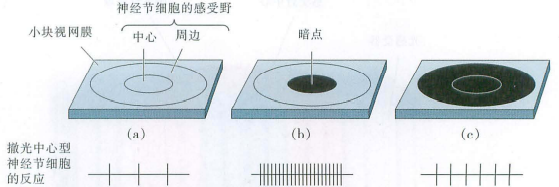
\includegraphics[width=.8\textwidth]{img/pic7-1.png}
                \caption{神经节细胞的中心-周边感受野\label{pic7-1}}
            \end{figure}
            \tiny{
                当一个暗点投射在撤光中心型神经节细胞的感受野中心时,细胞发放一串动作电位,但暗点范围扩大,则放电大幅减少。
            }
        % }
    % \end{columns}
    
\end{frame}

\begin{frame}
    \frametitle{神经节细胞感受野对明暗边界的调制}
    考察明暗边界对撤光中心神经节细胞输出的影响。根据实验,该信号有如图\ref{pic7-2}所示反应。%#TODO:做个图像分析
    \begin{figure}
        \centering
        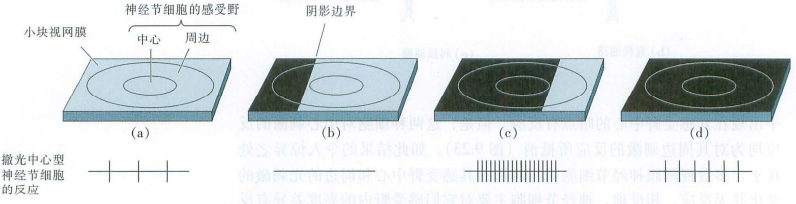
\includegraphics[width=.8\textwidth]{img/pic7-2.png}
        \caption{神经节细胞对感受野内明暗边界的反应\label{pic7-2}}
    \end{figure}
    从神经节细胞感受野的组织形式,我们可以推断,世界系统特化为对局部空间变化进行检测,而不是对于落在视网膜上光的绝对幅度进行检测,因此,\textbf{视网膜对光或暗的感知是相对的}。
\end{frame}
\subsection{神经细胞的类型}
在哺乳类视网膜,多数数神经节细胞具有一个中心-周边感受野,其中心
区域或具给光反应或具撒光反应。他们可以进一步根据外形、突触连接、和
电生理特性进行分类。

譬如,基于胞体大小与树突结构
\subsection{并行处理}